\documentclass{standalone}
\usepackage{tikz}
\usetikzlibrary{patterns, positioning}
\usepackage[sfdefault]{ClearSans} %% option 'sfdefault' activates Clear Sans as the default text font
\usepackage[T1]{fontenc}

\begin{document}
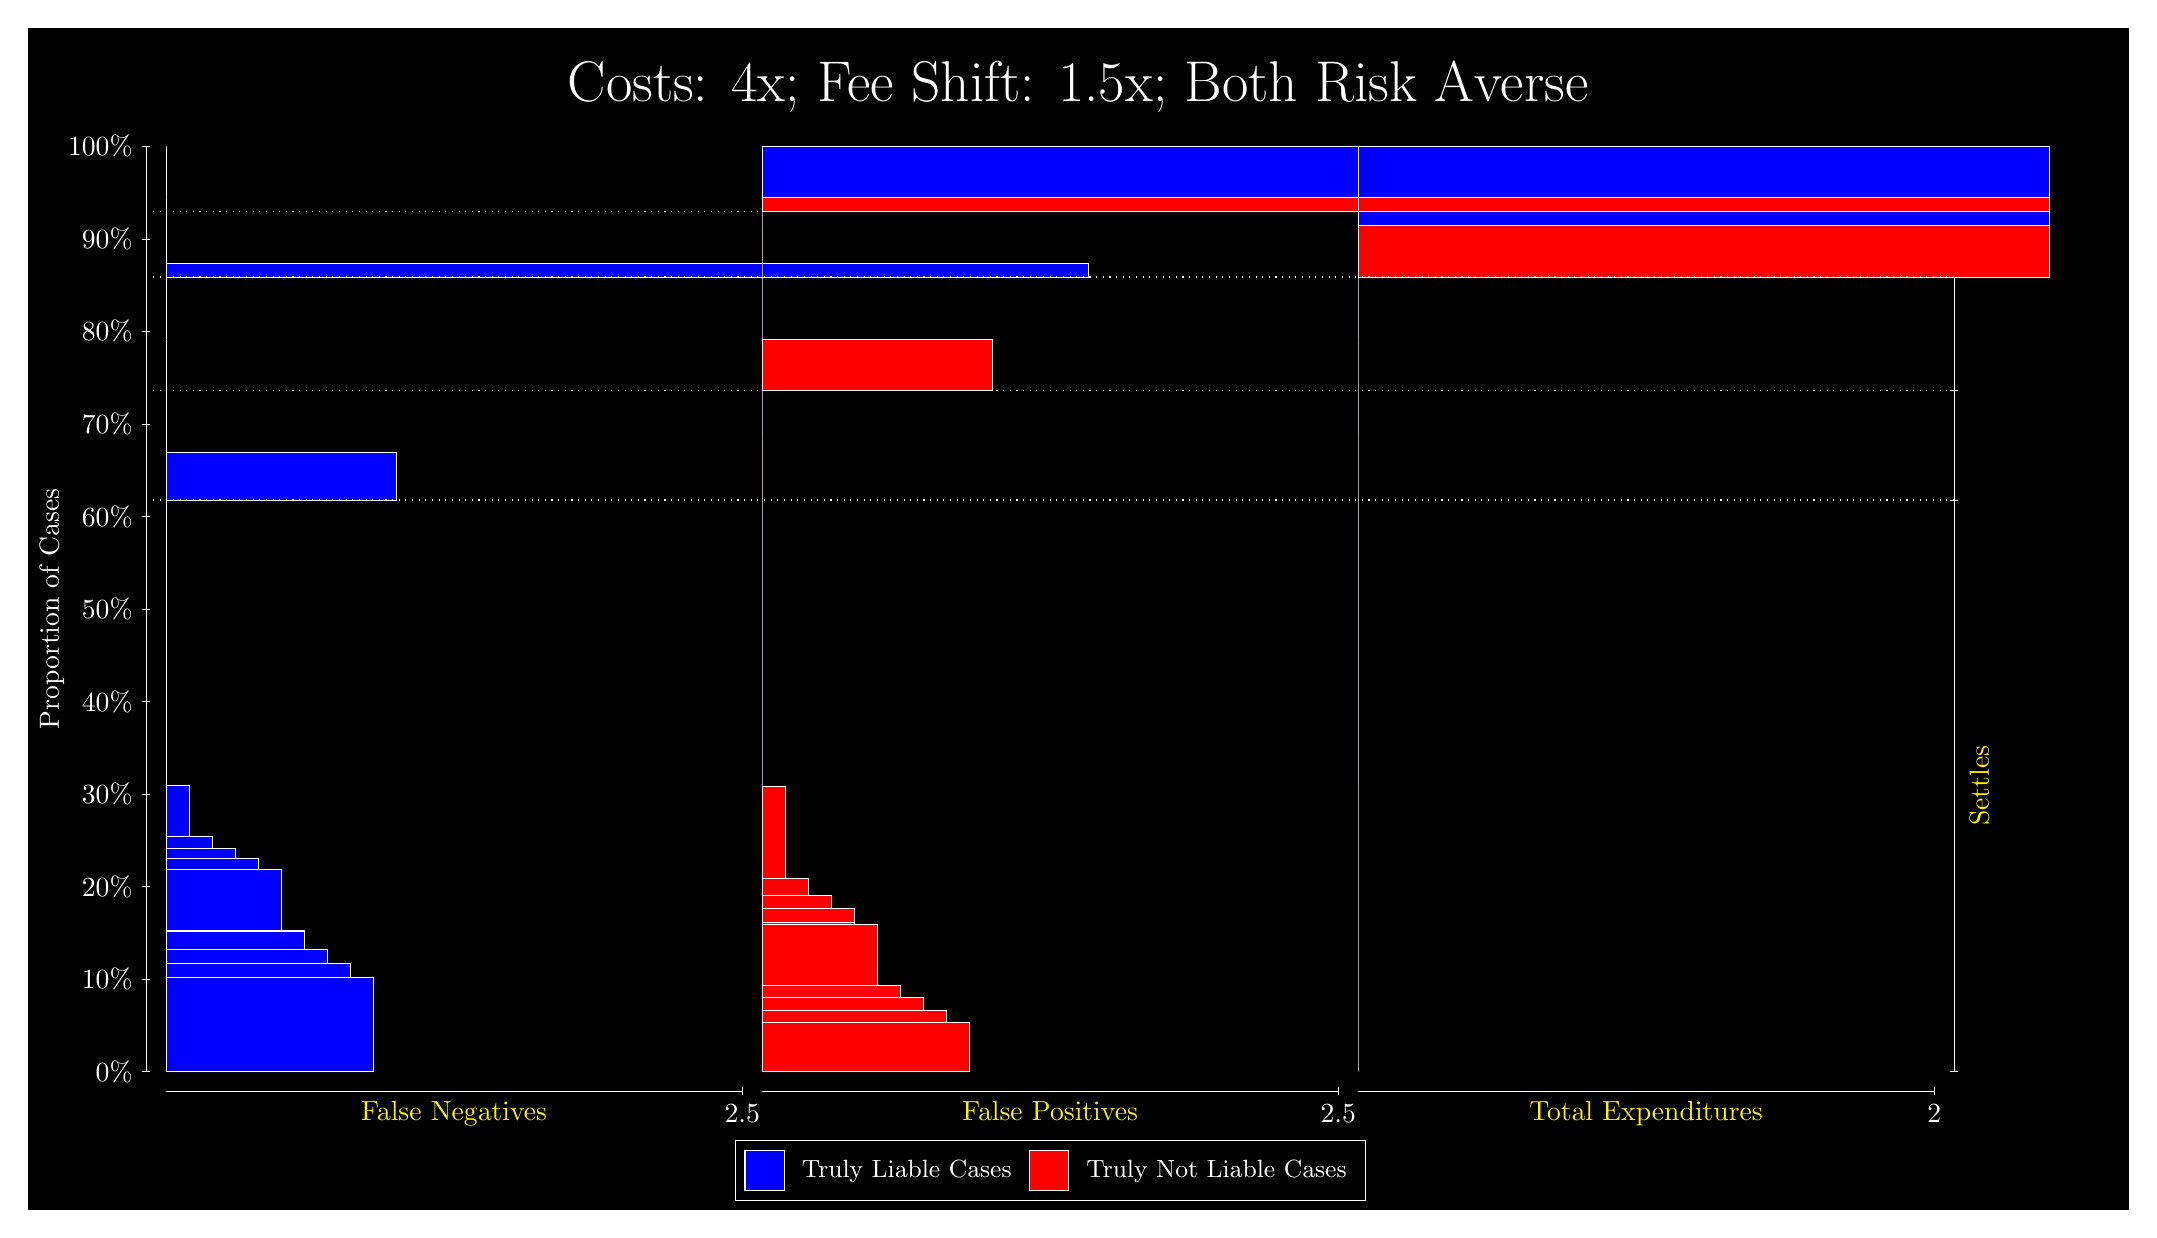
\begin{tikzpicture}
\draw[fill=black] (0,0) rectangle (26.667,15);
\draw[text=white] (0,13.5) rectangle (26.667,15) node[midway] {\huge Costs: 4x; Fee Shift: 1.5x; Both Risk Averse};
\draw[white, very thin] (1.5,1.75) -- (1.5,13.5);
\node[rotate=90, text=white, anchor=center] at (0.3, 7.625) {Proportion of Cases};
\draw[white, very thin] (1.45,1.75) -- (1.55,1.75);
\node[text=white, anchor=east] at (1.45, 1.75) {0\%};
\draw[white, very thin] (1.45,2.925) -- (1.55,2.925);
\node[text=white, anchor=east] at (1.45, 2.925) {10\%};
\draw[white, very thin] (1.45,4.1) -- (1.55,4.1);
\node[text=white, anchor=east] at (1.45, 4.1) {20\%};
\draw[white, very thin] (1.45,5.275) -- (1.55,5.275);
\node[text=white, anchor=east] at (1.45, 5.275) {30\%};
\draw[white, very thin] (1.45,6.45) -- (1.55,6.45);
\node[text=white, anchor=east] at (1.45, 6.45) {40\%};
\draw[white, very thin] (1.45,7.625) -- (1.55,7.625);
\node[text=white, anchor=east] at (1.45, 7.625) {50\%};
\draw[white, very thin] (1.45,8.8) -- (1.55,8.8);
\node[text=white, anchor=east] at (1.45, 8.8) {60\%};
\draw[white, very thin] (1.45,9.975) -- (1.55,9.975);
\node[text=white, anchor=east] at (1.45, 9.975) {70\%};
\draw[white, very thin] (1.45,11.15) -- (1.55,11.15);
\node[text=white, anchor=east] at (1.45, 11.15) {80\%};
\draw[white, very thin] (1.45,12.325) -- (1.55,12.325);
\node[text=white, anchor=east] at (1.45, 12.325) {90\%};
\draw[white, very thin] (1.45,13.5) -- (1.55,13.5);
\node[text=white, anchor=east] at (1.45, 13.5) {100\%};

\draw[white, very thin] (24.457,1.75) -- (24.457,13.5);
\draw[white, very thin] (24.407,1.75) -- (24.507,1.75);
\node[anchor=west] at (24.407, 1.75) {};
\draw[white, very thin] (24.407,9.0079) -- (24.507,9.0079);
\node[anchor=west] at (24.407, 9.0079) {};
\draw[white, very thin] (24.407,10.399) -- (24.507,10.399);
\node[anchor=west] at (24.407, 10.399) {};
\draw[white, very thin] (24.407,11.84) -- (24.507,11.84);
\node[anchor=west] at (24.407, 11.84) {};
\draw[white, very thin] (24.407,12.672) -- (24.507,12.672);
\node[anchor=west] at (24.407, 12.672) {};
\draw[white, very thin] (24.407,13.5) -- (24.507,13.5);
\node[anchor=west] at (24.407, 13.5) {};

\draw[white, very thin, fill=blue] (1.75,1.75) rectangle (4.3848,2.9416);
\draw[white, very thin, fill=blue] (1.75,2.9416) rectangle (4.092,3.1267);
\draw[white, very thin, fill=blue] (1.75,3.1267) rectangle (3.7993,3.3048);
\draw[white, very thin, fill=blue] (1.75,3.3048) rectangle (3.5065,3.5281);
\draw[white, very thin, fill=blue] (1.75,3.5281) rectangle (3.5065,3.5499);
\draw[white, very thin, fill=blue] (1.75,3.5499) rectangle (3.2138,4.3216);
\draw[white, very thin, fill=blue] (1.75,4.3216) rectangle (2.921,4.4526);
\draw[white, very thin, fill=blue] (1.75,4.4526) rectangle (2.6283,4.5865);
\draw[white, very thin, fill=blue] (1.75,4.5865) rectangle (2.3355,4.7423);
\draw[white, very thin, fill=blue] (1.75,4.7423) rectangle (2.0428,5.3895);
\draw[white, very thin, fill=red] (1.75,5.3895) rectangle (1.75,9.0079);
\draw[white, very thin, fill=blue] (1.75,9.0079) rectangle (4.6775,9.6204);
\draw[white, very thin, fill=red] (1.75,9.6204) rectangle (1.75,10.399);
\draw[white, very thin, fill=red] (1.75,10.399) rectangle (1.75,11.046);
\draw[white, very thin, fill=blue] (1.75,11.046) rectangle (1.75,11.84);
\draw[white, very thin, fill=blue] (1.75,11.84) rectangle (13.46,12.017);
\draw[white, very thin, fill=red] (1.75,12.017) rectangle (1.75,12.672);
\draw[white, very thin, fill=red] (1.75,12.672) rectangle (1.75,12.848);
\draw[white, very thin, fill=blue] (1.75,12.848) rectangle (1.75,13.5);
\draw[white, very thin, fill=red] (9.3189,1.75) rectangle (11.954,2.3757);
\draw[white, very thin, fill=red] (9.3189,2.3757) rectangle (11.661,2.534);
\draw[white, very thin, fill=red] (9.3189,2.534) rectangle (11.368,2.687);
\draw[white, very thin, fill=red] (9.3189,2.687) rectangle (11.075,2.851);
\draw[white, very thin, fill=red] (9.3189,2.851) rectangle (10.783,3.6174);
\draw[white, very thin, fill=red] (9.3189,3.6174) rectangle (10.49,3.6414);
\draw[white, very thin, fill=red] (9.3189,3.6414) rectangle (10.49,3.8221);
\draw[white, very thin, fill=red] (9.3189,3.8221) rectangle (10.197,3.9893);
\draw[white, very thin, fill=red] (9.3189,3.9893) rectangle (9.9044,4.2015);
\draw[white, very thin, fill=red] (9.3189,4.2015) rectangle (9.6116,5.3684);
\draw[white, very thin, fill=blue] (9.3189,5.3684) rectangle (9.3189,9.0079);
\draw[white, very thin, fill=red] (9.3189,9.0079) rectangle (9.3189,9.7863);
\draw[white, very thin, fill=blue] (9.3189,9.7863) rectangle (9.3189,10.399);
\draw[white, very thin, fill=red] (9.3189,10.399) rectangle (12.246,11.046);
\draw[white, very thin, fill=blue] (9.3189,11.046) rectangle (9.3189,11.84);
\draw[white, very thin, fill=red] (9.3189,11.84) rectangle (9.3189,12.495);
\draw[white, very thin, fill=blue] (9.3189,12.495) rectangle (9.3189,12.672);
\draw[white, very thin, fill=red] (9.3189,12.672) rectangle (21.029,12.848);
\draw[white, very thin, fill=blue] (9.3189,12.848) rectangle (18.102,13.5);
\draw[white, very thin, fill=red] (16.888,1.75) rectangle (16.888,5.3684);
\draw[white, very thin, fill=blue] (16.888,5.3684) rectangle (16.888,9.0079);
\draw[white, very thin, fill=red] (16.888,9.0079) rectangle (16.888,9.7863);
\draw[white, very thin, fill=blue] (16.888,9.7863) rectangle (16.888,10.399);
\draw[white, very thin, fill=red] (16.888,10.399) rectangle (16.888,11.046);
\draw[white, very thin, fill=blue] (16.888,11.046) rectangle (16.888,11.84);
\draw[white, very thin, fill=red] (16.888,11.84) rectangle (25.67,12.495);
\draw[white, very thin, fill=blue] (16.888,12.495) rectangle (25.67,12.672);
\draw[white, very thin, fill=red] (16.888,12.672) rectangle (25.67,12.848);
\draw[white, very thin, fill=blue] (16.888,12.848) rectangle (25.67,13.5);
\draw[white, dotted] (1.5,9.0079) -- (24.457,9.0079);
\draw[white, dotted] (1.5,10.399) -- (24.457,10.399);
\draw[white, dotted] (1.5,11.84) -- (24.457,11.84);
\draw[white, dotted] (1.5,12.672) -- (24.457,12.672);
\draw[white, very thin] (1.75,1.5) -- (9.0689,1.5);
\node[text=yellow, anchor=north] at (5.4094, 1.5) {False Negatives};
\draw[white, very thin] (9.0689,1.45) -- (9.0689,1.55);
\node[text=white, anchor=north] at (9.0689, 1.45) {2.5};

\draw[white, very thin] (9.3189,1.5) -- (16.638,1.5);
\node[text=yellow, anchor=north] at (12.978, 1.5) {False Positives};
\draw[white, very thin] (16.638,1.45) -- (16.638,1.55);
\node[text=white, anchor=north] at (16.638, 1.45) {2.5};

\draw[white, very thin] (16.888,1.5) -- (24.207,1.5);
\node[text=yellow, anchor=north] at (20.547, 1.5) {Total Expenditures};
\draw[white, very thin] (24.207,1.45) -- (24.207,1.55);
\node[text=white, anchor=north] at (24.207, 1.45) {2};

\node[text=yellow, centered, rotate=90] at (24.777, 5.379) {Settles};





\draw (12.978300999999998,1.5) node[draw=none] (baseCoordinate) {};
\begin{scope}[align=center]
        \matrix[scale=0.5, draw=white, below=0.5cm of baseCoordinate, nodes={draw}, column sep=0.1cm]{
            \node[rectangle, draw, minimum width=0.5cm, minimum height=0.5cm, fill=blue] {}; &
            \node[draw=none, font=\small, text=white] (B) {Truly Liable Cases}; &
            \node[rectangle, draw, minimum width=0.5cm, minimum height=0.5cm, fill=red] {}; &
            \node[draw=none, font=\small, text=white] (B) {Truly Not Liable Cases}; \\
            };
\end{scope}

\end{tikzpicture}
\end{document}